% --------------------------------------------------------------------------------

\begin{exercise}

\phantom{}

\begin{enumerate}[label = \textbf{\alph*)}]
  \item Beweisen Sie die Aussage in Kapitel 1, Exercise 6 des Vorlesungsskriptes.
  \item Beweisen Sie die Aussage in Kapitel 1, Exercise 7 des Vorlesungsskriptes.
\end{enumerate}

\end{exercise}

% --------------------------------------------------------------------------------

\begin{solution}

\phantom{}

\begin{enumerate}[label = \textbf{\alph*)}]

  \item \phantom{}

  \begin{figure}[h!]
    \centering
    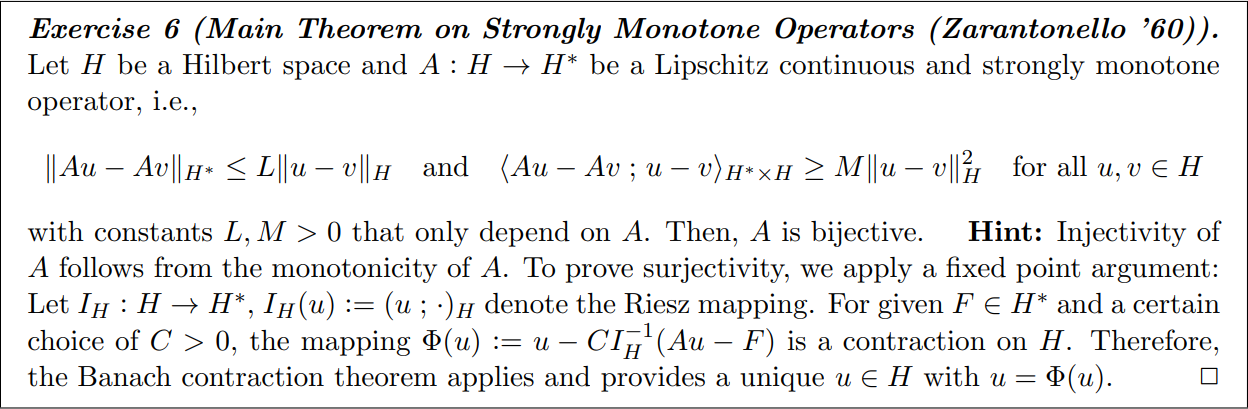
\includegraphics[width = 0.9 \textwidth]{../../../Fundament-LaTeX/images/NumPDEs/NumPDEs - Exercise 6 (Main Theorem on Strongly Monotone Operatos (Zarantonello '60)).png}
    \caption{Feischl \& Prätorius - Numerics of Partial Differential Equations: Stationary Problems}
  \end{figure}

  \begin{itemize}

    \item Injektivität:
    $\Forall u, v \in H:$

    \begin{align*}
      Au = Av
      \implies
      0 = \abraces{Au - Av; u - v}_{H^\ast \times H} \geq M \norm[H^2]{u -v}
      \implies
      u = v
    \end{align*}

    \item Surjektivität:
    Sei $I_H$ die bijektive Riesz-Abbildung.

    \begin{align*}
      I_H:
      H \to H^\ast:
      u \mapsto (u; \cdot)_H
    \end{align*}

    Für gegebenes $F \in H^\ast$ und einer noch offen zu wählendem $C > 0$ betrachten wir die Abbildung $\Phi$.

    \begin{align*}
      \Phi:
      H \to H:
      u \mapsto u - C I_H^{-1}(Au - F)
    \end{align*}

    Wir benützen die Stetigkeit und Monotonie von $A$, sowie die Linearität und Isometrie von $I_H^{-1}$ für folgende Rechnung.

    \begin{align*}
      \norm[H]{\Phi(u) - \Phi(v)}^2
      & =
      \norm[H]{u - C I_H^{-1}(Au - F) - v + C I_H^{-1}(Av - F)}^2 \\
      & =
      \norm[H]{u - v - C I_H^{-1}(Au - Av)}^2 \\
      & =
      \norm[H]{u - v}^2
      +
      \norm[H]{C I_H^{-1}(Av - Au)}^2
      -
      2 (u - v; C I_H^{-1}(Au - Av))_H \\
      & =
      \norm[H]{u - v}^2
      +
      C^2 \norm[H^\ast]{Au - Av}^2
      -
      2 C (I_H^{-1}(Au - Av); u - v)_H \\
      & \leq
      \norm[H]{u - v}^2
      +
      C^2 L^2 \norm[H]{u - v}^2
      -
      2 C I_H \pbraces{I_H^{-1}(Av - Au)}(v - u) \\
      & =
      \norm[H]{u - v}^2
      +
      C^2 L^2 \norm[H]{u - v}^2
      -
      2 C \abraces{Av - Au; v - u} \\
      & \leq
      \norm[H]{u - v}^2
      +
      C^2 L^2 \norm[H]{u - v}^2
      -
      2 C M \norm[H]{u - v}^2 \\
      & =
      \norm[H]{u - v}^2 (1 + C^2 L^2 - 2CM)
    \end{align*}

    Damit ist $\Phi$ eine Kontraktion genau dann, wenn

    \begin{multline*}
      0 \leq \sqrt{1 + C^2 L^2 - 2CM} < 1
      \iff
      1 + C^2 L^2 - 2CM < 1
      \iff
      C^2 L^2 - 2CM < 0 \\
      \iff
      C^2 L^2 < 2CM
      \iff
      C L^2 < 2M
      \iff
      C < \frac{2M}{L^2}.
    \end{multline*}

    Ein solches $C$ existiert, und damit, nach dem Banachschen Fixpunktsatz, $\ExistsOnlyOne u \in H:$

    \begin{align*}
      u = \Phi(u) = u - C I_H^{-1}(Au - F)
      \implies
      I_H^{-1}(Au - F) = 0
      \implies
      Au = F.
    \end{align*}

  \end{itemize}

  \item \phantom{}

  \begin{figure}[h!]
    \centering
    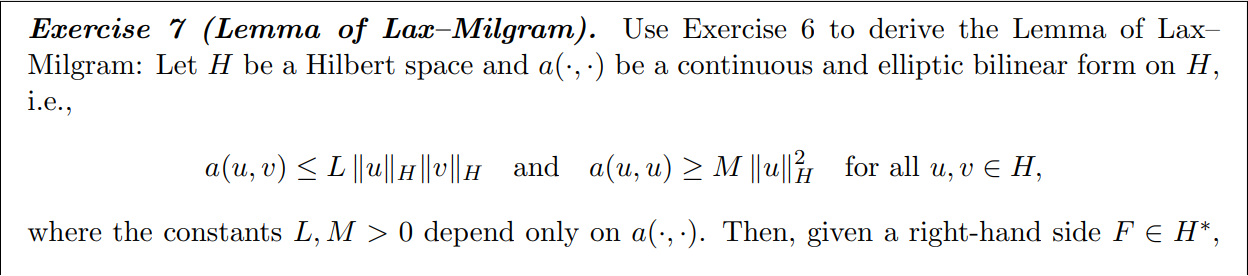
\includegraphics[width = 0.9 \textwidth]{../../../Fundament-LaTeX/images/NumPDEs/NumPDEs - Exercise 7.1 (Lemma of Lax-Milgram).png}
    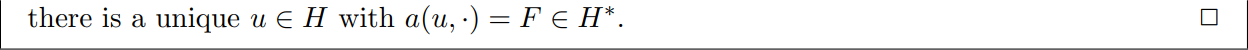
\includegraphics[width = 0.9 \textwidth]{../../../Fundament-LaTeX/images/NumPDEs/NumPDEs - Exercise 7.2 (Lemma of Lax-Milgram).png}
    \caption{Feischl \& Prätorius - Numerics of Partial Differential Equations: Stationary Problems}
  \end{figure}

  Wir betrachten einen geeigneten Operator $A$, auf den wir a) anwenden wollen.

  \begin{align*}
    A:
    H \to H^\ast:
    u \mapsto a(u, \cdot).
  \end{align*}

  $A$ ist offensichtlich linear.

  \begin{itemize}

    \item Lipschitz-Stetigkeit:

    Seien $u, v \in H$.
    Weil $a$ stetig ist, gilt $\Forall w \in H:$

    \begin{align*}
      |(Au - Av)(w)|
      =
      |(Au)(w) - (Av)(w)|
      =
      |a(u, w) - a(v, w)|
      =
      |a(u - v, w)|
      \leq
      L \norm[H]{u - v} \norm[H]{w}
    \end{align*}

    Laut Definition der Operatornorm, ist als $\norm[H^\ast]{Au - Av} \leq L \norm[H]{u - v}$.

    \item Monotonie:

    Seien $u, v \in H$.
    Weil $a$ elliptisch ist, gilt

    \begin{align*}
      \abraces{Au - Av; u - v}_{H^\ast \times H}
      =
      a(u - v; u - v)
      \geq
      M \norm[H]{u - v}^2.
    \end{align*}

  \end{itemize}

  Also können wir Exercise 6 anwenden und erhalten

  \begin{align*}
    \Forall F \in H^\ast:
    \ExistsOnlyOne u \in H:
    a(u, \cdot) = F.
  \end{align*}

\end{enumerate}

\end{solution}

% --------------------------------------------------------------------------------
